% XXX Jedes Jahr Professoren-Texte aktualisieren!
\section[Eure Profs stellen sich vor]{Eure Professoren stellen sich vor}
\textbf{Auf den folgenden zwei Seiten stellen sich eure beiden Professoren vor.
    Sie werden gemeinsam die "Physik~1" bis "Physik~3" lesen.
    Prof.\ Doltsinis wird sich dabei um die theoretischen und Prof.\ Kohl um die experimentellen Aspekte des Studiums kümmern.
    Zudem stellt sich Prof.\ Wulkenhaar vor, der die Vorlesungen "Mathematik für Physiker" halten wird (ebenfalls über drei Semester).
	Da diese drei Professoren euch eine Zeit lang begleiten werden, ist es durchaus mal interessant zu wissen, was sie gemacht haben, bevor sie an die Uni Münster kamen, und wie ihre aktuelle Forschung aussieht.}

\begin{multicols}{2}
\begin{center}
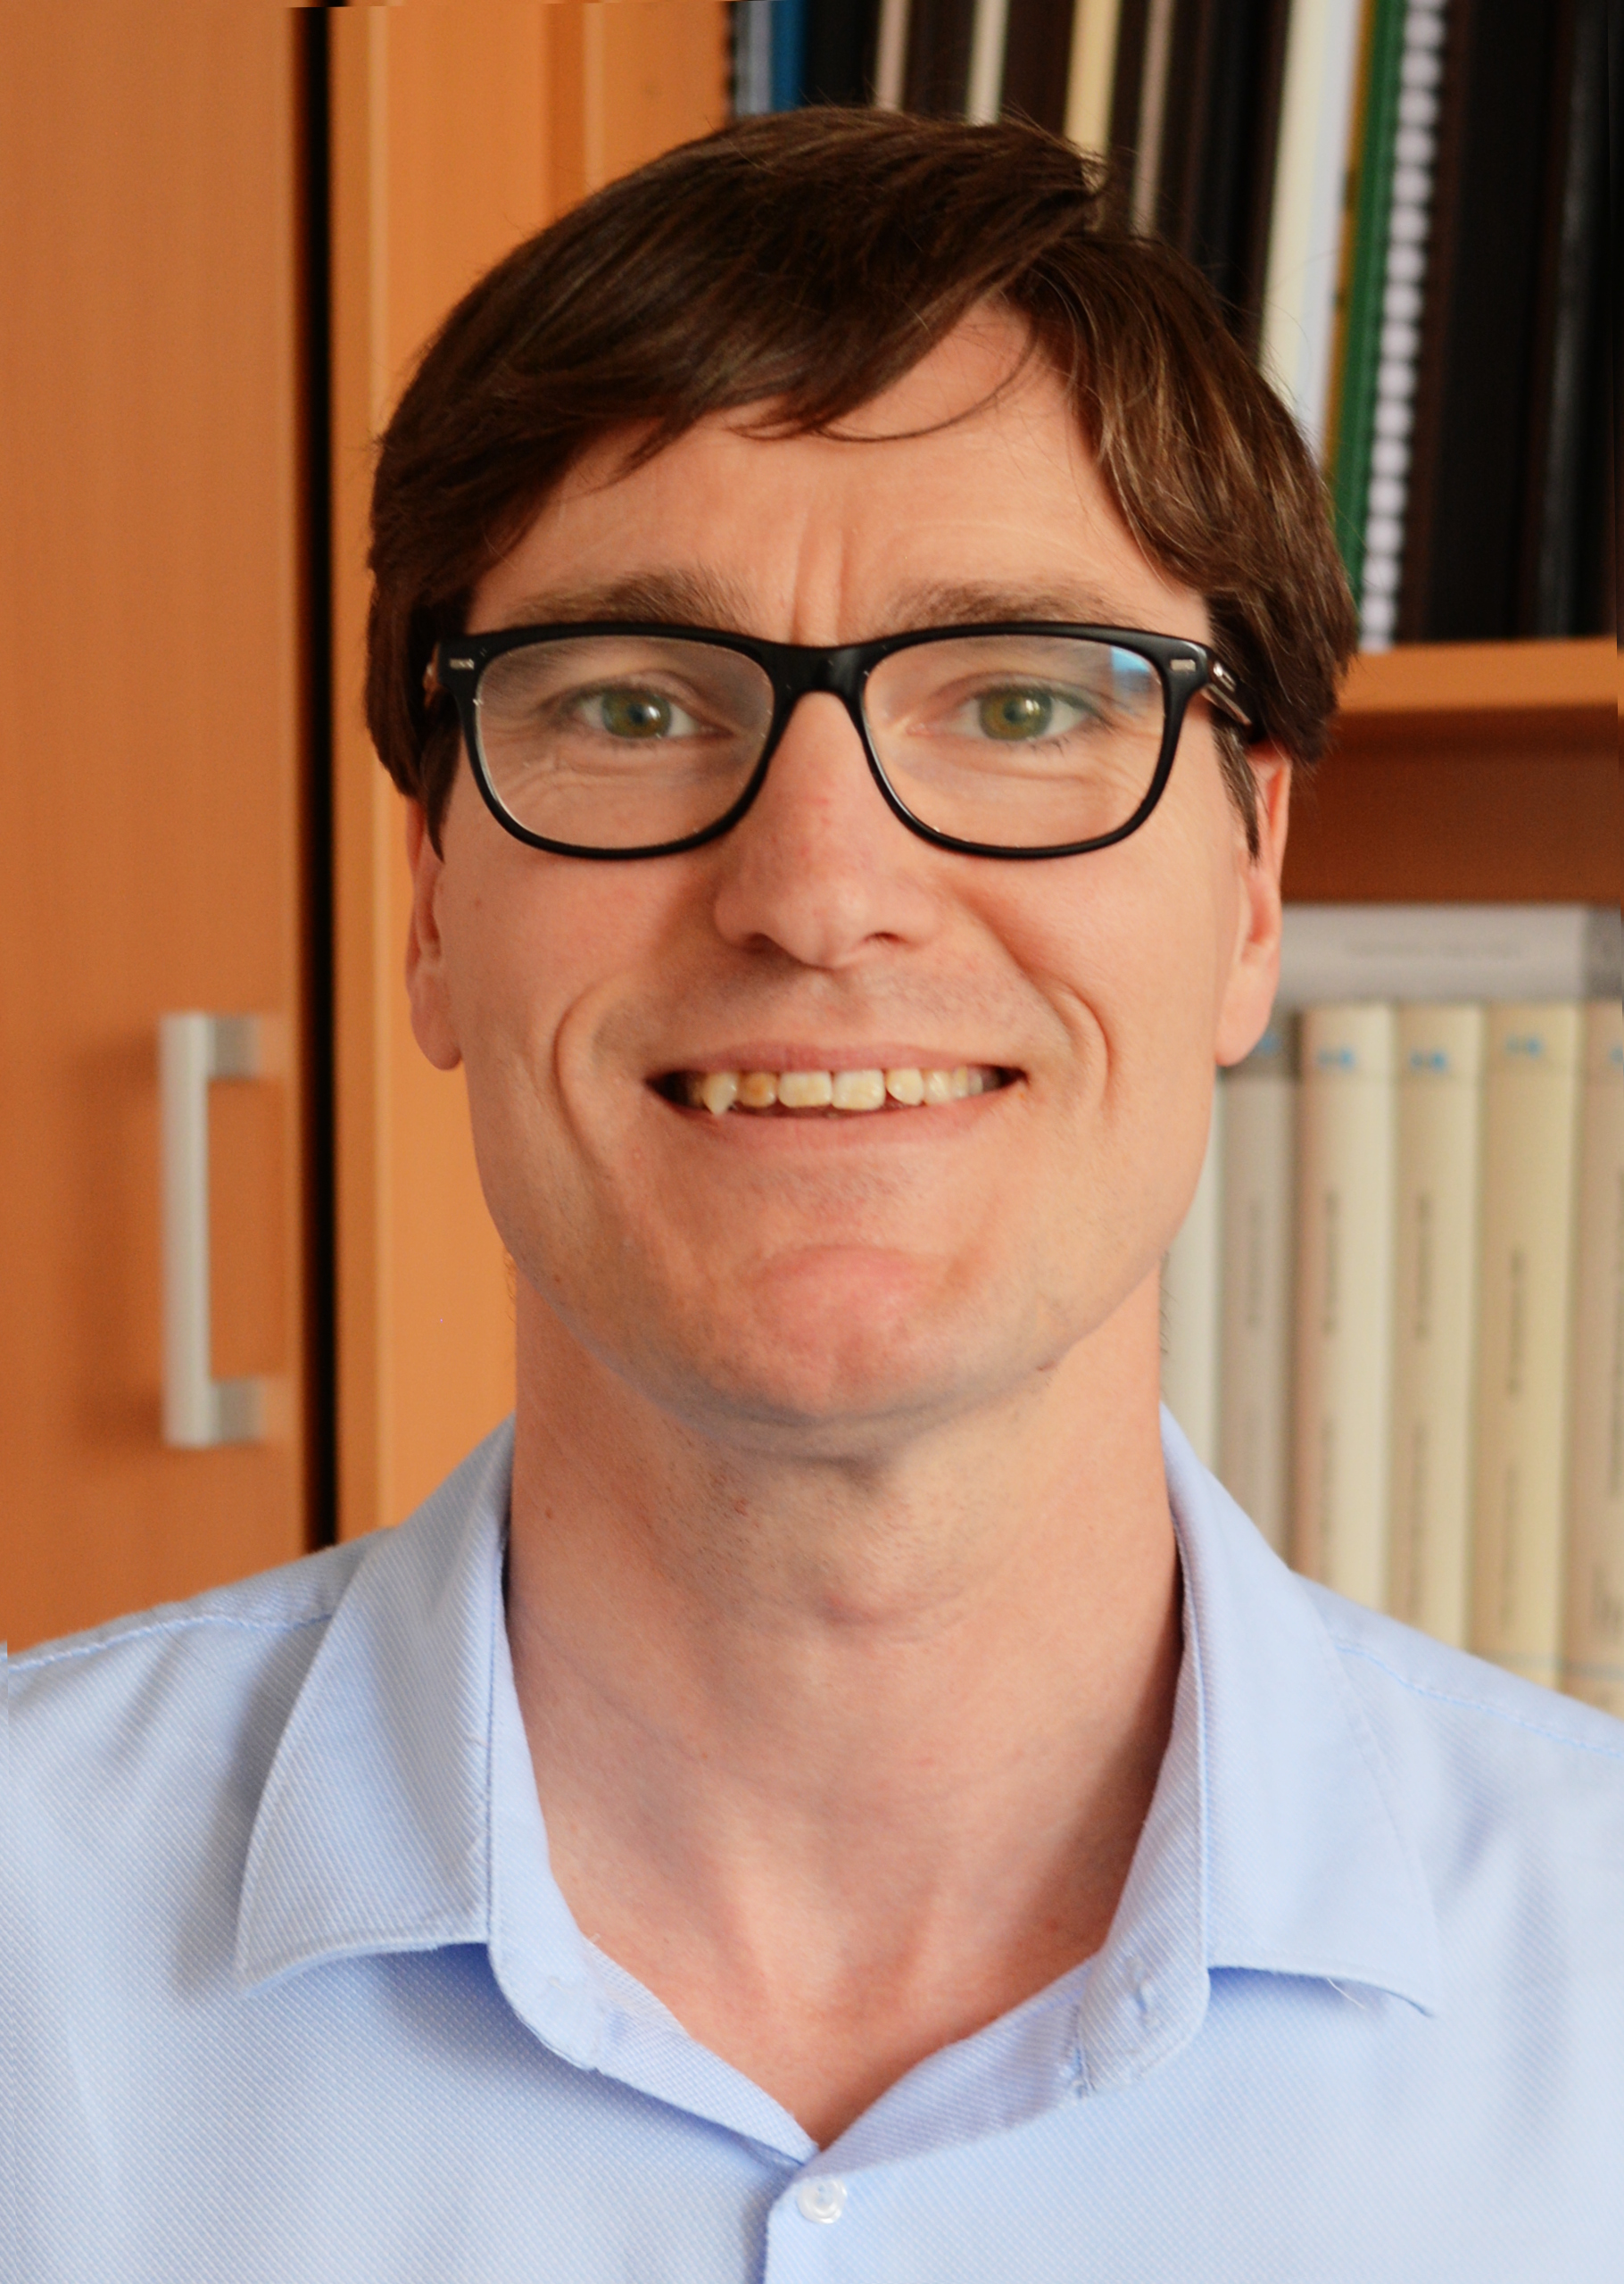
\includegraphics[width=0.8\columnwidth]{res/vorstellungsfotos/doltsinis.jpg}\\
\smallskip
Prof.\ Dr.\ Nikos\ Doltsinis\\
Institut für Festkörpertheorie
\end{center}

Seit dem Sommersemester 2011 bin ich Professor am Institut für Festkörpertheorie der Westfälischen Wilhelms-Universität Münster. Meine Forschungsinteressen liegen im Bereich der Computersimulation molekularer Materie, wobei deren Wechselwirkung mit Licht einen besonderen Schwerpunkt bildet.  Aktuelle Anwendungsgebiete beinhalten z.B. die Entwicklung organischer Solarzellen, organischer lichtemittierender Dioden (OLEDs) sowie molekularer Motoren. Sie können sich jetzt schon darauf freuen, im Rahmen Ihrer Bachelorarbeit (üblicherweise im 6. Semester) an solchen oder ähnlichen spannenden Fragestellungen in einer der Arbeitsgruppen im Fachbereich Physik selbst aktiv mitzuforschen. Auf dem Weg dahin werden meine Kollegen und ich Ihnen die nötigen physikalischen Grundlagen vermitteln. In den nächsten drei Semestern werde ich Sie, gemeinsam mit meinem Kollegen Prof. Dr. Helmut Kohl, durch die Module Physik I-III führen, die die Gebiete Mechanik, Thermodynamik, Elektrodynamik, Optik und Relativitätstheorie umfassen. Dem WWU-spezifischen Konzept des “integrierten Kurses” folgend werden wir experimentelle und theoretische Aspekte Hand-in-Hand vorstellen, wobei ich für den theoretischen Teil zuständig bin. 

Exakt vor 30 Jahren war ich, wie Sie jetzt, Studienanfänger im Fach Physik an der Universität Stuttgart. Nach dem Erhalt meines Physik-Diploms im Jahr 1995 wechselte ich nicht nur die Universität und das Land, sondern auch das Fach. Ich ging nach England an die Universität Birmingham, wo ich im Jahr 1998 im Fach Theoretische Chemie promovierte. Im Anschluss forschte ich zwei Jahre lang als Postdoktorand an der Universität Cambridge, bevor ich nach Deutschland zurückkehrte und mich im Jahr 2007 an der Universität Bochum habilitierte. Meine erste Festanstellung als “Lecturer” bekam ich kurz darauf am King’s College London, wo ich 2009 zum “Senior Lecturer” befördert wurde. Schließlich nahm ich im Jahr 2011 den Ruf auf eine Professur für die Theorie funktionaler Nanostrukturen an der WWU an.  

\end{multicols}

\newpage

\begin{multicols}{2}
\begin{center}
	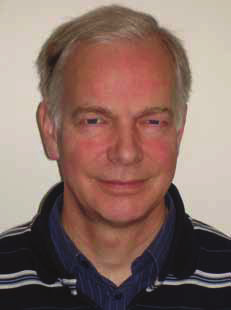
\includegraphics[width=\columnwidth, height=0.35\textheight]{res/vorstellungsfotos/kohl.jpg}\\
\smallskip
	Prof.\ Dr.\ Helmut\ Kohl\\
	Physikalisches Institut
\end{center}

In den nächsten drei Semestern werden wir uns gemeinsam im „Integrierten Kurs“ (Physik 1-3) mit den Grundlagen der Physik befassen. Darauf freue ich mich sehr. Ich bin dabei für den experimentellen Teil verantwortlich.

Kurz zu meinem Werdegang: Nach meinem Abitur habe ich Physik an der Technischen Hochschule Darmstadt studiert und 1980 mein Diplom abgeschlossen. Drei Jahre später habe ich über die „Abbildung mit unelastisch gestreuten Elektronen in der hochauflösenden Elektronenmikroskopie“ promoviert. Danach war ich zu einem einjährigen Forschungsaufenthalt am Laboratoire de Physique des Solides der Université Paris-Sud. Neben der wissenschaftlichen Tätigkeit habe ich dabei auch das Leben in einem anderen Land kennengelernt. Mit einigen meiner damaligen Kolleginnen und Kollegen habe ich bis heute freundschaftlichen Kontakt.

Anschließend kehrte ich an die TH Darmstadt zurück, wo ich mich 1989 habilitierte. Nach Aufenthalten an der Technischen Universität Wien und dem Max-Planck Institut für Metallforschung in Stuttgart wurde ich 1993 an die Westfälische Wilhelms-Universität Münster berufen und leite hier die Abteilung „Elektronenmikroskopie“ im Physikalischen Institut.  Gemeinsam mit Gruppen aus den Instituten für Materialphysik, für Mineralogie, für Planetologie und dem Geologisch-Paläontologischen Institut betreiben wir das Interdisziplinäre Centrum für Elektronenmikroskopie und Mikroanalyse (ICEM).

In der Elektronenmikroskopie ist es durch die Verwendung von unelastisch gestreuten Elektronen beispielsweise möglich, die Elementverteilung in einem Festkörper mit einer Ortsauflösung von etwa einem Nanometer (10-9 m) abzubilden. Dies ist von großer praktischer Bedeutung, sowohl in der Forschung, als auch in der Industrie. In unserer Arbeitsgruppe befassen wir uns mit den Grundlagen derartiger Techniken u.a. mit dem Ziel, Auflösungs- und Nachweisgrenzen weiter  zu verbessern und die Genauigkeit bei der quantitativen Auswertung zu steigern. Für mich liegt der besondere Reiz dieses Gebiets in der Verknüpfung von grundlegenden Fragen der Quantenmechanik mit praktischen Anwendungen.

Im Rahmen der Vorlesungen wird es um die Grundlagen der Physik gehen, insbesondere auch in Verbindung mit experimentellen Messmethoden. Vermutlich wird Ihnen der Wechsel von der Schule an die Universität nicht ganz leicht fallen. Dennoch hoffe ich, dass Sie weiter Freude am Fach Physik haben werden.   

Für Fragen oder Anregungen zu Vorlesung oder Übungen können Sie mich gerne nach einer Vorlesung oder in meinem Büro (R. 323) ansprechen.

\begin{center}
\includegraphics[width=0.85\columnwidth]{private/res/comics/teleskop.png}
\end{center}
\end{multicols}

\newpage

\begin{multicols}{2}
\begin{center}
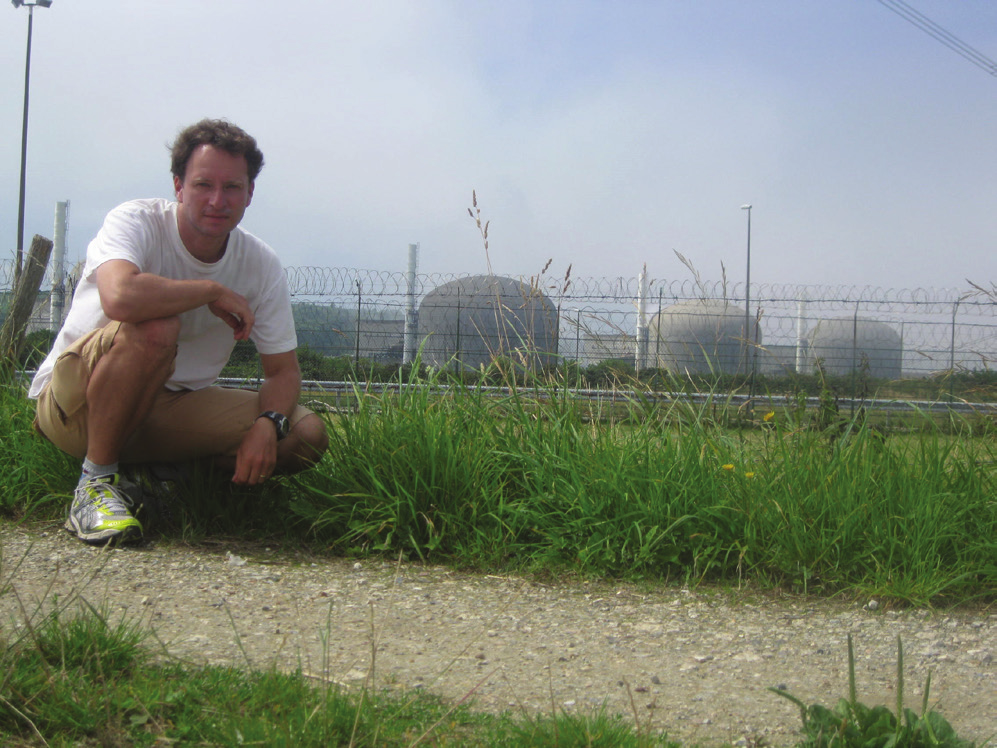
\includegraphics[width=0.9\columnwidth]{res/vorstellungsfotos/wulkenhaar.png}\\
Prof.\ Dr.\ Raimar Wulkenhaar\\
Mathematisches Institut
\end{center}

Ich bin von der Ausbildung her Physiker, arbeite im Grenzgebiet zwischen Mathematik und Physik und bin seit 2005 Professor für Reine Mathematik am Fachbereich Mathematik und Informatik der WWU.

Die Vorlesung "Mathematik für Physiker" wird traditionell vom Mathematischen Institut veranstaltet. Ich selbst werde den Zyklus zum 7.~Mal halten. Es ist aus meiner Sicht eine schöne Vorlesung; mir ist aber klar, dass die meisten Studierenden das anders sehen.

Auch wenn der Stoff durchaus umfangreich ist, können wir nur einen kleinen Teil dessen behandeln, was die Physik benötigt. Es geht in der Vorlesung nicht um die Bereitstellung von Rechenwerkzeugen für die Physik; das bekommen Sie nebenbei in den Physikvorlesungen geliefert. Es geht in der Mathematik darum zu verstehen, weshalb diese Rechenwerkzeuge so und nicht anders funktionieren. Der Einstieg in die Denkweise der Mathematik ist für viele nicht leicht. Erst im Lauf der Zeit entsteht rückblickend ein gewisses Verständnis für die tiefliegenden Strukturen und Zusammenhänge der Mathematik. Im Idealfall gelangen Sie so zu einer soliden Grundlage, mit der Sie die Rechenwerkzeuge der Physik nicht nur verstehend nutzen, sondern kreativ weiterentwickeln können.


\[
\resizebox{0.45\hsize}{!}{$\displaystyle\sum_{n = 1}^\infty \frac{1}{n^2} = \frac{\pi^2}{6}$}
\]

Nun noch einige Informationen zu mir. Nach Physikistudium an der Universität Leipzig mit Abschluss als Diplomphysiker. 1994 habe ich in Leipzig auch meine Doktorarbeit geschrieben und 1997 verteidigt. Dabei ging es um die Formulierung von Modellen der Teilchenphysik im Rahmen der nichtkommutativen Geometrie. Die Ergebnisse sind rückblickend völlig unwichtig, sie haben mich aber 1998/1999 als DAAD-Postdoc nach Marseille gebracht.

Ich habe am Centre de Physique Theorique in Marseille mein Arbeitsgebiet gefunden, die Quantenfeldtheorie auf nichtkommutativen Geometrien. Vereinfacht gesagt geht es um die Frage (und ihre Konsequenzen), ob man auf beliebig kleinen Längenskalen, sagen wir $10^{-80}$\,m, noch Physik betreiben kann. Es gibt gute Gründe anzunehmen, dass das unmöglich ist, und entsprechend sollte zur Formulierung physikalischer Gesetze eine Geometrie benutzt werden, in der $10^{-80}$\,m ebenfalls sinnlos sind. Diese Nichtkommutative Geometrie wird in einer Sprache analog zur Quantenphysik beschrieben.

Seit Marseille, vor allem aber seit meiner zweiten Postdoc-Station 2000/2001 an der Universität Wien, arbeite ich an quantenfeldtheoretischen Modellen auf einer besonders einfachen nichtkommutativen Geometrie. Während meines dritten Postdoc-Aufenthalts 2002/2005 am Max- Planck-Institut für Mathematik in den Naturwissenschaften in Leipzig konnte ich mit meinem Kollegen aus Wien zusammen eine größere Hürde beseitigen. Die mathematisch rigorose Konstruktion einer 4-dimensionalen Quantenfeldtheorie auf einer nichtkommutativen Geometrie konnten wir inzwischen abschließen. Etwas analoges ist in der üblichen kommutativen Geometrie bisher nicht geglückt. Es resultierten spannende Fragen, an denen ich seitdem arbeite.

\begin{center}
\includegraphics[width=0.85\columnwidth]{private/res/comics/calvin_mathe.pdf}
\end{center}
\end{multicols}
